\begin{figure}[H]
    \centering
    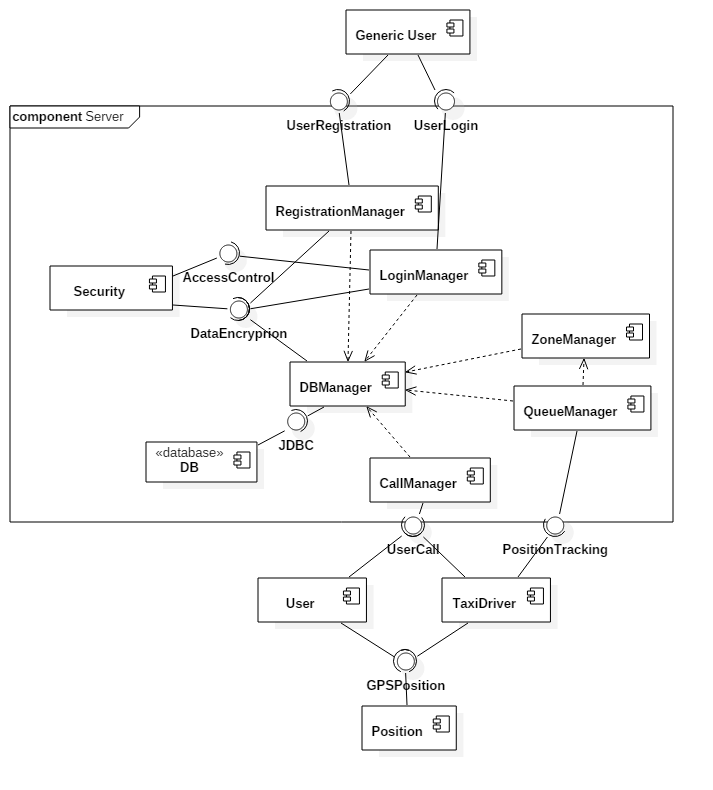
\includegraphics[width=14cm]{./Images/ComponentDiagram.png}
    \caption{Component diagram of our system}
    \label{fig:component-diagram}
\end{figure}


\subparagraph{Account Manager}
This component handles the account of a user providing two different interfaces in order to allow all the users to manage their account. One interface is used by the taxi driver and the other by the other users.
This component manages:
\begin{itemize}
    \item Modification of personal data.
    \item Modification of the account's password.
    \item Visualization of the list of old requests.
    \item Modification of the status of a taxi driver.
\end{itemize}

\subparagraph{Database Manager}
This component manages the interaction with the database providing all the information asked by all the other components.

\subparagraph{Zone Manager}
This component coordinates all the zones the city is divided in.
\begin{itemize}
    \item It create the queues of every zone.
    \item When a taxi driver leaves a queue, the QueueManager notifies this component and it searches the taxi driver associating it to a new queue.
\end{itemize}

\subparagraph{Queue Manager}
This component manages the taxi drivers in a certain zone.
\begin{itemize}
    \item Add/delete a taxi driver from the queue
    \item Change the position of taxi drivers in the queues.
    \item When a request is incoming it searches for the right taxi driver to send the request to.
\end{itemize}

\subparagraph{Call Manager}
This component manages all the incoming/waiting calls for a taxi.
\begin{itemize}
    \item Retrieves all the information regarding the call.
    \item Updates the information of the calls when their status is changed.
\end{itemize}

\subparagraph{Position}
The scope of this component is to get the GPS positions of all the taxi drivers and send the information to the QueueManager, and get the position of a user mobile phone who is creating a call request and send it to the CallManager.

\subparagraph{Security}
This component offers some interfaces to grant security to the whole system.
